In this section we provide a quick review about scintillators and the relevant electronic devices for this experiment. We also discuss a simple model for positrons in metals.

\subsection{Scintillator}
Scintillation counters detect ionizing particles. The particles excite molecules in the scintillator material. After a mean excitation time an excited molecule falls back into the groundstate and emits a photon with the corresponding wavelength. This photon can excite other molecules and performs kind of a random walk. To interrupt this random walk the scintillator material can be weakly doped with wavelength changing elements, e.g.\ with certain different molecules. Photons with the changed wavelength can no longer be absorbed by the original molecules and can leave the scintillator material. With an optical fibre the signal gets to a photodiode which generates and amplifies an electric signal which can be measured. The process is sketched in figure \ref{fig:scintillator}.
\begin{figure}[h]
  \centering
  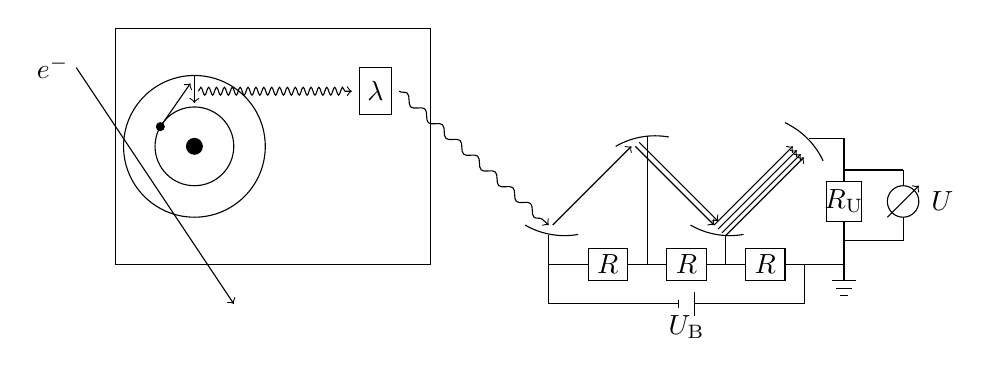
\begin{tikzpicture}[photon1/.style={decorate,decoration={snake, segment length=1mm, amplitude=0.5mm, post length=0.5mm}},photon2/.style={decorate,decoration={snake, segment length=3mm, amplitude=0.5mm, post length=0.5mm}}]
    \draw (0,0) rectangle (4,3);
    \draw [->] (-0.5,2.5)--(1.5,-0.5);
    \draw (-0.8,2.5) node {$e^-$};
    \draw (1,1.5) circle (0.9);
    \draw (1,1.5) circle (0.5);
    \draw [fill=black] (1,1.5) circle (0.1);
    \draw [fill=black] (1-0.5*1.732/2,1.5+1/4) circle (0.05);
    \draw [->] (1-0.5*1.732/2,1.5+1/4)--(0.95,2.3);
    \draw [->] (1,2.4) -- (1,2.05);
    \draw [->,photon1] (1.05,2.2) -- (3,2.2);
    \draw (3.1,1.9) rectangle (3.5,2.5);
    \draw (3.3,2.2) node {$\lambda$};
    \draw [->,photon2] (3.6,2.2)-- (5.5,0.5);
    \draw (5.2,0.5) arc (-120:-80:1);
    \draw [->] (5.55,0.5) -- (6.55,1.5);
    \draw (6.35,1.5) arc (120:80:1);
    \draw [->] (6.6,1.5) -- (7.6,0.5);
    \draw [->] (6.65,1.55) -- (7.65,0.55);
    \draw (7.3,0.5) arc (-120:-80:1);
    \draw [->] (7.65,0.45) -- (8.65,1.45);
    \draw [->] (7.6,0.5) -- (8.6,1.5);
    \draw [->] (7.7,0.4) -- (8.7,1.4);
    \draw [->] (7.74,0.36) -- (8.74,1.36);
    \draw (8.5,1.8) arc (65:25:1);
    \draw (9,0)--(8.5,0);
    \draw (8.75,0)--(8.75,-0.5)--(7.35,-0.5);
    \draw (7.15,-0.5)--(5.5,-0.5)--(5.5,0);
    \draw (8.5,0.2) rectangle (8,-0.2);
    \draw (8.25,0) node {$R$};
    \draw (8,0) -- (7.5,0);
    \draw (7.5,0.2) rectangle (7,-0.2);
    \draw (7.25,0) node {$R$};
    \draw (7,0) -- (6.5,0);
    \draw (7.75,0)--(7.75,0.375);
    \draw (6.75,0)--(6.75,1.635);
    \draw (6.5,0.2) rectangle (6,-0.2);
    \draw (6.25,0) node {$R$};
    \draw (6,0)--(5.5,0)--(5.5,0.375);
    \draw (7.35,-0.65)--(7.35,-0.35);
    \draw (7.15,-0.55)--(7.15,-0.45);
    \draw (7.25,-0.8) node {$U_\mathrm{B}$};
    \draw (9,0)--(9.25,0)--(9.25,0.55);
    \draw (9.03,0.55) rectangle (9.47,1.05);
    \draw (9.25,0.8) node {$R_\mathrm{U}$};
    \draw (9.25,1.05)--(9.25,1.6)--(8.8,1.6);
    \draw (9.25,0)--(9.25,-0.2);
    \draw (9.1,-0.2)--(9.4,-0.2);
    \draw (9.15,-0.3)--(9.35,-0.3);
    \draw (9.2,-0.4)--(9.3,-0.4);
    \draw (9.25,0.3)--(10,0.3);
    \draw (9.25,1.2)--(10,1.2);
    \draw (10,0.8) circle (0.2);
    \draw (10,0.3)--(10,0.6);
    \draw (10,1.2)--(10,1);
    \draw [->] (9.8,0.6)--(10.2,1);
    \draw (10.5,0.8) node {$U$};
  \end{tikzpicture}
  \caption{Example for the creation of a signal in a scintillator.}
  \label{fig:scintillator}
\end{figure}

In this experiment the scintillator is driven by high-voltage. This increases the time resolution. For signals which get used for time measurements we measure the signal at the anode (fast-signal). If one needs a better energy resolution one measures the signal at one of the photo dynodes (slow-signal).\\ \\
The scintillator material used in this experiment is LYSO. The scintillator has an intrinsic spectrum due to the decay of $^{176}$Lu. 
\subsection{Electronic Components}

\subsubsection*{Single-Channel Analyzer and Coincidence Circuit}
Single-channel analyzers (SCA) transform analog signals in the set range to digital signals. We will use them to single out signals coming from specific peaks of the emission spectrum.\\ \\
For lifetime measurements we are interested in signals which come (nearly) at the same time. To single out such signals one uses a coincidence circuit. This has two analog inputs and a digital output. The function of the coincidence circuit is that of a logical AND.
\subsubsection*{Multichannel Analyzer}
For the recording of spectra we use a multichannel analyer (MCA). The MCA has an digital input for the gate signal and one analog input for the signal with the information about the bin in which the signal gets sorted in. The bins are seperated equidistant with respect to the amplitude of the incoming signal.

\subsubsection*{Time-Analog-Converter}
With the time-analog-converter (TAC) one can measure the time difference between two digital signals. The TAC has two analog inputs, one for the start-signal and one for the stop-signal. The time difference of the signals is proportional to the analog signal of the output.

\subsubsection*{Constant-Fraction Discriminator}
For the lifetime measurement we use constant-fraction discriminators (CFD) to transform the analog signal of the scintillator to a digital signal which we use for the lifetime measurement. The reason for not using a SCA is that the SCA transforms signals only differing in the scaling of the amplitude to digital signals at different times. The CFD does not have this problem since it gives out the analog signal when a set fraction of the amplitude is reached. For this procedure to work there exists of course a maximal time duration for the incoming signal.

\subsection{Positrons in Metals}
In the discussion of a model for positrons in metals we completely follow \cite{material_tutor}. In the presented model there are two possible states for positrons in metal (after thermalization). They can either be moving freely like the electrons or they can be trapped in vacancies. Both states are not stable and after a mean lifetime the positron will annihilate with an electron. The mean lifetime for positrons moving freely (being trapped) is denoted by $\tau_\mathrm{f}$ ($\tau_\mathrm{t}$). Following \cite{material_tutor} the lifetimes fulfill $\tau_\mathrm{f}< \tau_\mathrm{t}$. The rate of free positrons getting trapped can be described by the constant rate $\sigma$ and the density of vacancies $\rho$.  We do not consider trapped positrons becoming free. 

\begin{figure}[h]
  \centering
  \begin{tikzpicture} [photon/.style={decorate,decoration={snake, segment length=2mm, amplitude=0.5mm, post length=0.5mm}}]
    \draw(0,0)--(5,0) node [right] {$n_\mathrm{t}$};
    \draw(0,2)--(5,2) node [right] {$n_\mathrm{f}$};
    \draw [->] (-1,2.8)--(0.2,2.1);
    \draw (-0.9,3.1) node {e$^+$};
    \draw (-1.8,2.5) node {thermalization};
    \draw [->] (1.5,1.9)--(1.5,0.1); 
    \draw (1.5,1) node [left] {$\sigma \rho$};
    \draw [->,photon] (3.5,0.1)--(4.5,1.1);
    \draw (4.1,0.6) node [right] {$\tau_\mathrm{t}$};
    \draw [->,photon] (3.5,2.1)--(4.5,3.1);
    \draw (4.1,2.6) node [right] {$\tau_\mathrm{f}$};
  \end{tikzpicture}
  \caption{Decay of positrons in metal.}
  \label{fig:model}
\end{figure}

The resulting differential equations for the number of free and trapped positrons are given by
\begin{align*}
  \diff{n_\mathrm{f}}{t}&=-\frac{n_\mathrm{f}}{\tau_\mathrm{f}}-\sigma \rho n_\mathrm{f}\\
  \diff{n_\mathrm{t}}{t}&=-\frac{n_\mathrm{t}}{\tau_t}+\sigma \rho n_\mathrm{f}.
\end{align*}
Solving these equations with the initial condition $n_\mathrm{t}(0)=0$ and $n_\mathrm{f}(0)=n_0$ one finds that the rate for the annihilation radiation is given by
\begin{align*}
  W(t)=-\frac{1}{n_0}\diff{}{t} (n_\mathrm{f}+n_\mathrm{t})=\frac{I_0}{\tau_0}e^{-t/\tau_0}+\frac{I_\mathrm{t}}{\tau_\mathrm{t}}e^{-t/\tau_\mathrm{t}}
\end{align*}
with
\begin{align*}
  \tau_0&=\left( \frac{1}{\tau_\mathrm{f}}+\sigma\rho\right)^{-1}\\
  I_0&=\frac{1/\tau_\mathrm{f}-\tau_0/\tau_\mathrm{t}(1/\tau_\mathrm{f}+\sigma\rho)}{1/\tau_0-1/\tau_t}\\   I_\mathrm{t}&=1-I_0.     
\end{align*}
In practice we need to take into account that any measured time difference is smeared out by a resolution function. According to \cite{further_instructions} the general form of the lifetime spectrum $N(t)$ which is the convolution of the annihilation radiation rate and the resolution function with an additive offset then has the form
\begin{align}
  N(t)=\sum_{i\in\{ 0,\mathrm{t}\}}\frac{A_i}{2\tau_i}e^{\frac{\sigma^2-2\tau_i(t-t_0)}{2\tau_i^2}}(\mathrm{erf}(a_i)+\mathrm{erf}(b_i))+BG
\label{eq:fit_rate}
\end{align}  
with
\begin{align*}
  a_i&=\frac{\sigma^2+\tau_it_0}{\sqrt{2}\sigma\tau_i}\\
  b_i&=\frac{\tau_i(t-t_0)-\sigma^2}{\sqrt{2}\sigma\tau_i}.
\end{align*}
The intensities can then be expressed by
\begin{align*}
  I_i=\frac{A_i}{A_0+A_\mathrm{t}}.
\end{align*}
The mean lifetime and the lifetime of the free state can be calculated according to 
\begin{align*}
  \bar{\tau}&=I_o\tau_0+ I_\mathrm{t}\tau_\mathrm{t}\\
  \tau_\mathrm{f}&=\left( I_0/\tau_0 + I_\mathrm{t}/\tau_\mathrm{t}\right)^{-1}.
\end{align*}
With the knowledge of $\bar{\tau}$, $\tau_\mathrm{f}$ and $\tau_\mathrm{t}$ one can calculate the transition rate by
\begin{align}
  \sigma \rho= \frac{\bar{\tau}-\tau_\mathrm{f}}{\tau_\mathrm{f}(\tau_\mathrm{f}-\bar{\tau})}.
\label{eq:transition_rate}
\end{align}
Since the transition rate depends on the temperature $T$ and the vacancy formation enthalpy $H_\mathrm{t}$ with
\begin{align}
  \sigma \rho=\sigma \exp\left(\frac{S_\mathrm{t}}{k_B}\right)\exp\left({-\frac{H_\mathrm{t}}{k_\mathrm{B}T}}\right),
  \label{eq:enthalpy}	
\end{align}
where $k_\mathrm{B}$ is the Boltzmann constant and for indium (see \cite{weiler})
\begin{align*}
  \sigma \exp\left( \frac{S_\mathrm{t}}{k_B}\right)=10^8/\si{\nano\second}
\end{align*}
one can calculate the vacancy formation enthalpy by fitting the lifetime spectrum for different temperatures.

\subsection{Decay Schemes of $^{127}$Lu and $^{22}$Na}
The decay schemes of $^{127}$Lu and $^{22}$Na can be found in figure \ref{fig:scheme}. 
\begin{figure}[h]
  \centering
  \begin{subfigure}[h]{0.5\textwidth}
    \centering
    \includegraphics[width=0.9\textwidth]{Figures/LuScheme.png}
  \end{subfigure}%
  \begin{subfigure}[h]{0.5\textwidth}
    \centering
    \includegraphics[width=0.7\textwidth]{Figures/NaScheme.png}
  \end{subfigure}
  \caption{Decay schemes of $^{127}$Lu and $^{22}$Na from \cite{further_instructions}.}
  \label{fig:scheme}
\end{figure}   

\newpage
